\documentclass[11pt]{standalone}
\usepackage{amssymb}
\usepackage{amsmath}
\usepackage[no-math]{fontspec}
\usepackage{unicode-math}
\usepackage{libertinus}
\usepackage{pgf,xcolor}
\usepackage{tikz}
\usetikzlibrary{arrows.meta, backgrounds}
\usepackage{pgfplots}
\pgfplotsset{compat=newest}

\definecolor{my_darkgray}{HTML}{484949}
\definecolor{my_lightgray}{HTML}{F3F4F4}
\definecolor{my_darkblue}{HTML}{005A94}
\definecolor{my_lightblue}{HTML}{CCDEE9}
\definecolor{my_yellow}{HTML}{FFEC7F}
\definecolor{my_red}{HTML}{E60000}
\definecolor{my_orange}{HTML}{E87846}

%% Fourier series (Papula convention): f(t) = -1 on [-pi,0), f(t) = +1 on [0,pi)
%%   b_n = 4/(n*pi) for odd n,  b_n = 0 for even n
%%
%% Partial sums (x in radians):
%%   S_1 = (4/pi)*sin(x)
%%   S_3 = (4/pi)*sin(x) + (4/(3*pi))*sin(3*x)
%%   S_9 = (4/pi)*sin(x) + (4/(3*pi))*sin(3*x) + (4/(5*pi))*sin(5*x)
%%         + (4/(7*pi))*sin(7*x) + (4/(9*pi))*sin(9*x)
%%
%% Step function (const plot) over [-2*pi, 2*pi]:
%%   [-2pi, -pi): f = +1   (maps to [0, pi))
%%   [-pi,   0 ): f = -1
%%   [0,     pi): f = +1
%%   [pi,   2pi): f = -1   (maps to [-pi, 0))
%%
%% S_1 max amplitude: 4/pi ~= 1.273
%% Gibbs overshoot for S_9: ~= 1 + 0.089*2 ~= 1.18

\begin{document}
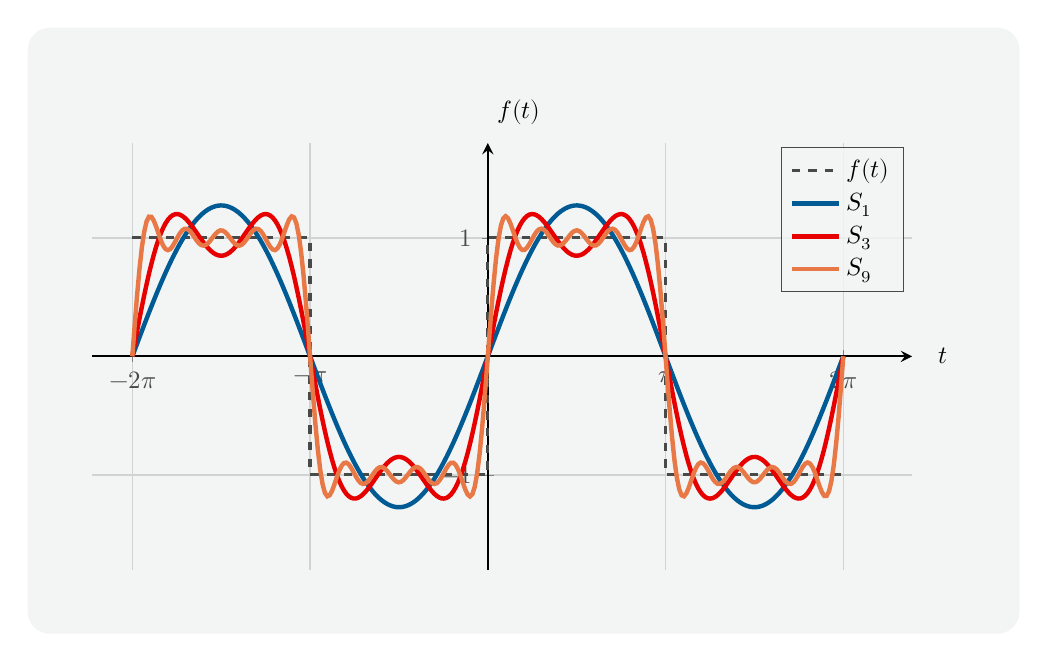
\begin{tikzpicture}[
    show background rectangle,
    background rectangle/.style={fill=my_lightgray, rounded corners=8pt},
    inner frame sep=0.8cm
]

\begin{axis}[
    axis lines = center,
    xlabel = {$t$},
    ylabel = {$f(t)$},
    xlabel style={at={(axis description cs:1.02,0.5)}, anchor=west, font=\small},
    ylabel style={at={(ticklabel* cs:1.02)}, anchor=south west, font=\small},
    xmin = -7.0,
    xmax = 7.5,
    ymin = -1.8,
    ymax = 1.8,
    xtick = {-6.28318, -3.14159, 0, 3.14159, 6.28318},
    xticklabels = {$-2\pi$, $-\pi$, $0$, $\pi$, $2\pi$},
    ytick = {-1, 0, 1},
    yticklabels = {$-1$, $0$, $1$},
    axis line style = {thick},
    grid = both,
    grid style = {draw=my_lightgray!60!white, line width=0.4pt},
    major grid style = {draw=my_lightgray!80!my_darkgray, line width=0.5pt},
    tick label style = {font=\small, color=my_darkgray},
    width = 12cm,
    height = 7cm,
    % axis equal not used: y-values are dimensionless +-1, x-values in radians
    legend style = {
        at={(0.99, 0.99)},
        anchor=north east,
        font=\small,
        fill=my_lightgray,
        draw=my_darkgray,
        fill opacity=0.85,
        text opacity=1,
    },
    legend cell align=left,
]

%% --- Rectangular target signal f(t) ---
\addplot[
    const plot,
    draw = my_darkgray,
    dashed,
    line width = 1.2pt,
    no marks,
]
coordinates {
    (-6.28318,  1)
    (-3.14159, -1)
    ( 0,        1)
    ( 3.14159, -1)
    ( 6.28318, -1)   %% terminates the last segment at 2*pi
};
\addlegendentry{$f(t)$}

%% --- S_1 = (4/pi)*sin(x) ---
\addplot[
    draw = my_darkblue,
    ultra thick,
    samples = 300,
    domain = -6.28318:6.28318,
]{
    (4/pi)*sin(deg(x))
};
\addlegendentry{$S_1$}

%% --- S_3 = (4/pi)*sin(x) + (4/(3*pi))*sin(3*x) ---
\addplot[
    draw = my_red,
    ultra thick,
    samples = 300,
    domain = -6.28318:6.28318,
]{
    (4/pi)*sin(deg(x))
    +(4/(3*pi))*sin(deg(3*x))
};
\addlegendentry{$S_3$}

%% --- S_9: terms for n = 1, 3, 5, 7, 9 ---
\addplot[
    draw = my_orange,
    ultra thick,
    samples = 300,
    domain = -6.28318:6.28318,
]{
    (4/pi)*sin(deg(x))
    +(4/(3*pi))*sin(deg(3*x))
    +(4/(5*pi))*sin(deg(5*x))
    +(4/(7*pi))*sin(deg(7*x))
    +(4/(9*pi))*sin(deg(9*x))
};
\addlegendentry{$S_9$}

\end{axis}

\end{tikzpicture}
\end{document}
